%--------------------------------------------------------------------------
% !TEX root = 5Blman.tex
% energy.tex
% 2012.12.27 changed to 2col format
%--------------------------------------------------------------------------
\chapter{Electric Energy}

%---------------------------------------------------------------------
\begin{multicols}{2}
\section{Purpose}
  The purpose of this laboratory exercise is to explore the relation between electrical energy and heat. You will find the energy transferred to a cup partially filled with water with a current passing through it.  The energy will be found using calorimetry methods and compared to electrical methods.  This lab will help you to understand concepts of energy and power associated with electric current and demonstrate the conversion of electrical energy to heat. You will also be able to describe what is meant by joule heat, explain the factors on which joule heat depends, and show how joule heat may be measured experimentally. The heat generated or power dissipated is referred to as joule heat.

%The purpose of this laboratory exercise is to describe what is meant by joule heat, explain the factors on which joule heat depends, and show how joule heat may be measured experimentally
\section{Preparation}
  Reread the sections in your text regarding electrical energy and power before coming to lab. Pay special attention to the relationship of voltage, current, and power.  You may also wish to review sections in your text on temperature change and specific heat.
%\paragraph{Short quiz }
% Be prepared to take a short quiz or hand in a prelab assignment at the beginning of lab related to the concepts of voltage, current, power, and energy.

%---------------------------------------------------------------------
\section{General Information}
Using your measured values of mass, temperature, voltage, current, and time you will calculate the energy put into a cup partially filled with water and associated material around it.  The energy will be calculated by two methods.  First by considerations of the energy needed to cause a temperature change and second by considerations of electrical energy.  The results of the two calculations should agree within experimental uncertainties if most or all of the energy put into the system by the electric current is retained as thermal energy in the system.  We thus verify that the energy associated with temperature change is the same as the energy associated with electric current. 
 \reffig{f:fig2} shows the basic set-up.  A DC power supply is connected to a coil of wire immersed in an aluminum cup partially filled with water.  (Not shown are the cup's lid, the stirring device, and the thermometer.)  The current is passed through an ammeter connected in series with the coil.  The voltage across the coil is measured by a voltmeter. %connected as shown.  
\paragraph{Caution}
Be sure you understand the operation of the various components in the circuit.  Do not turn on the power supply until the instructor has checked to see that the system is wired correctly.  The ammeter is particularly vulnerable to damage if improperly connected.  Also, do not turn on the current unless the heating coil is immersed in water or it may burn out or burn you.

\begin{center}
%\begin{figure}
%	\centering
	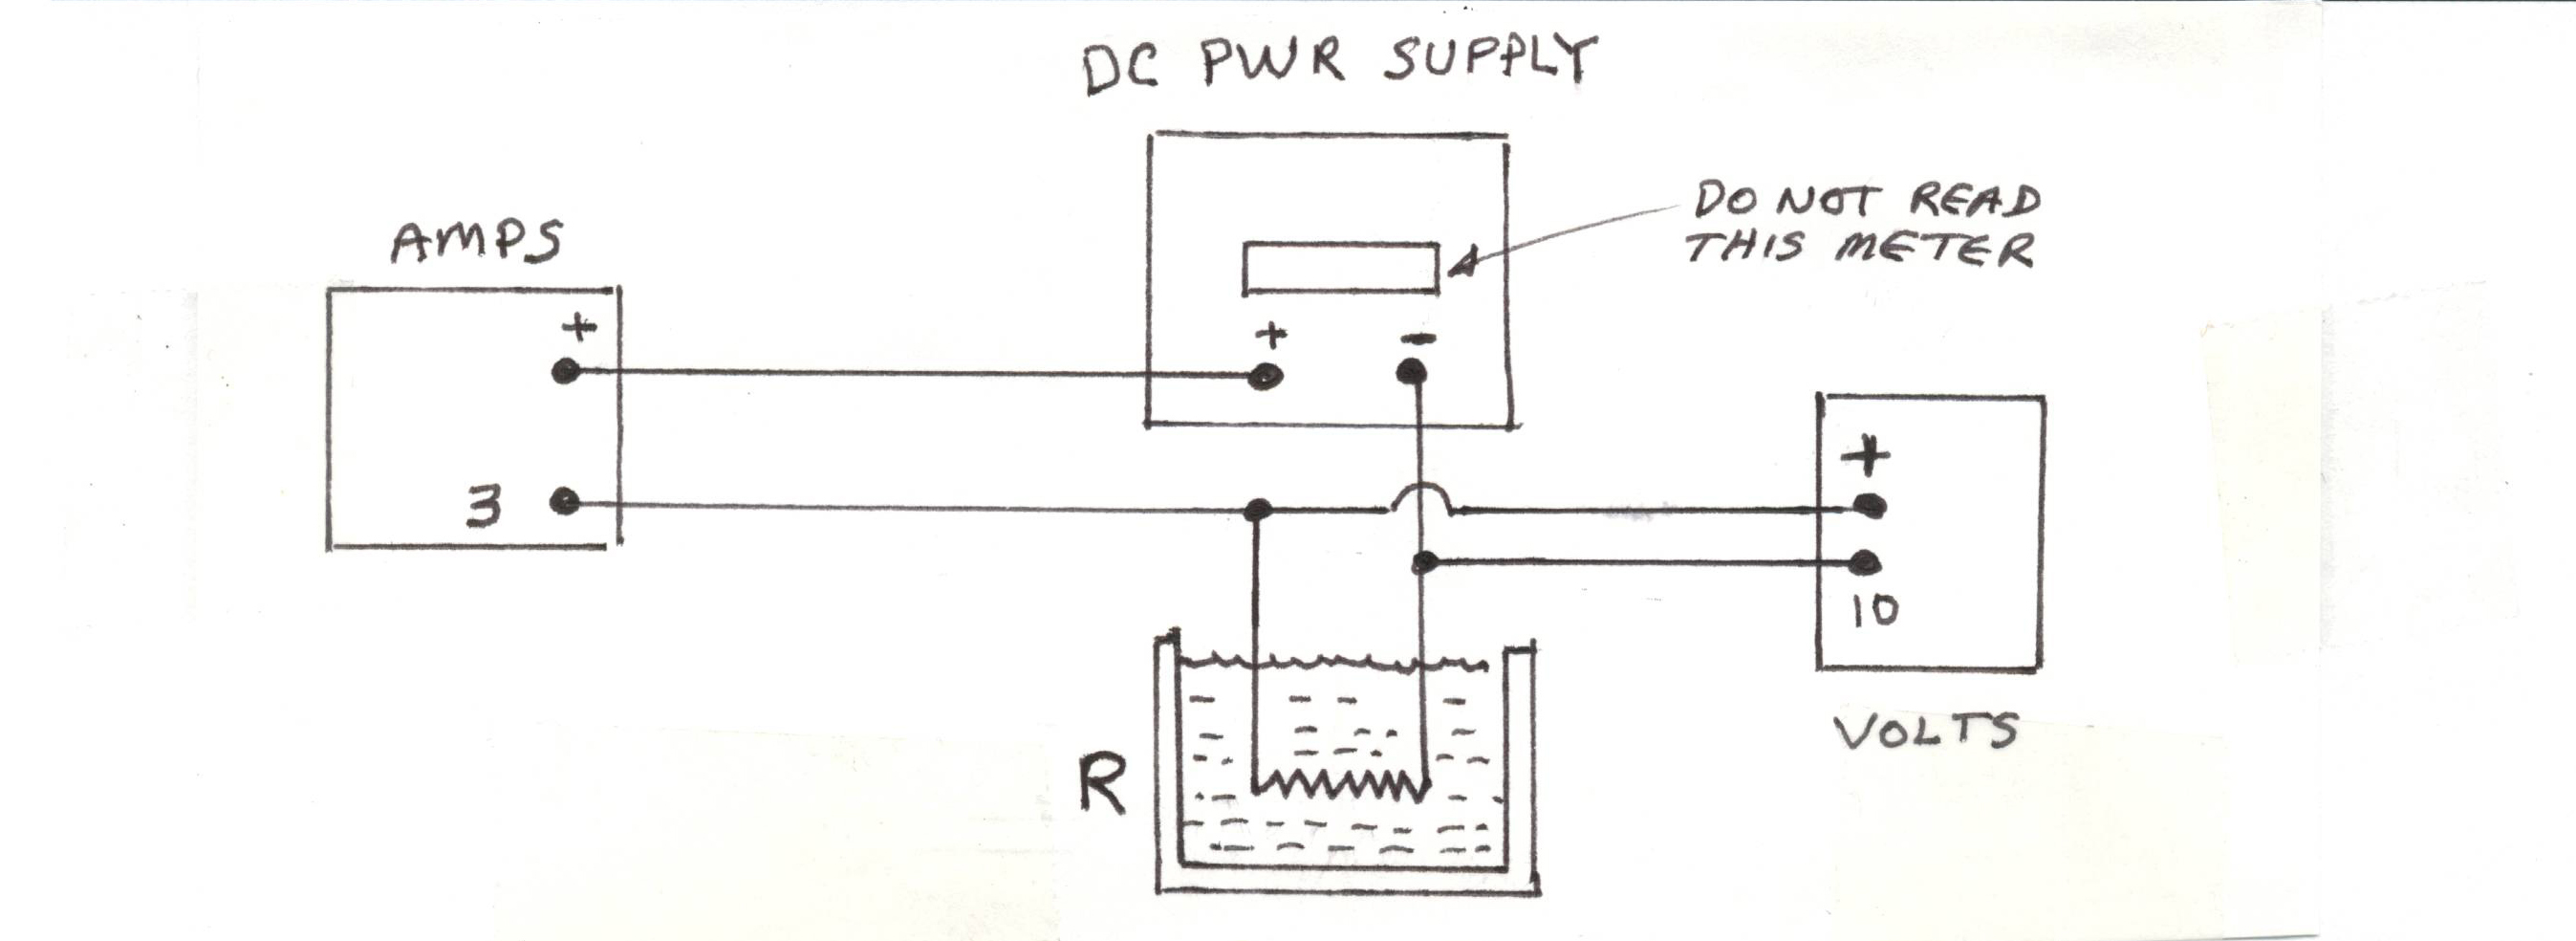
\includegraphics[scale=0.65]{5bgraf/fig_2}
%	\caption{Block diagram for calorimetry set-up}
	\mfcaption{Calorimetry set-up: block diagram}
	\label{f:fig2}
%\end{figure}
\end{center}

%\begin{center}
%	\includegraphics[scale=0.8]{5bgraf/fig_2b}
%	\mfcaption{Calorimetry set-up: schematic}
%	\label{f:fig3}
%\end{center}

%---------------------------------------------------------------------
\section{Theory}
To calculate the energy needed to heat the system by the calorimetry method we note that the amount of energy needed to increase the temperature of an object is
\begin{equation} \label{e:qheat1}
	Q = mc\Delta T 
\end{equation}
where $Q$ is the amount of heat, $m$ is the mass of the object, $c$ is its specific heat, and $\Delta T$ is the change in temperature, $\Delta T =T_2 - T_1$.  Since our system has more than one substance, the energy required is the sum of the energy needed for each substance in the system.

In this exercise we heat water in an aluminum cup.  But we also heat the coil of wire, stirrer, thermometer, and part of the lid and connecting rods.  This sounds complicated, but experimentation has determined that all of these other factors are equivalent to 6.00 cal/\si{\degree}C of water. Finally, we assume that everything that is heated has the same temperature change.  Therefore, the equation we use to calculate the energy input by the calorimetry method is
\begin{equation}\label{e:qheat2}
	Q = [m_wc_w + m_{Al}c_{Al} + m_{coil}c_{coil}](T_2 - T_1)
\end{equation}
where	
\begin{description}[itemsep=1pt]
	\item [$m_w$] = mass of water
	\item [$m_{Al}$]	= mass of Al calorimeter cup
	\item [$c_w$]	= specific heat of water (1.00 cal/g \si{\degree}C)
	\item [$c_{Al}$]	= specific heat of Al (0.22 cal/g \si{\degree}C)
	\item [$m_{coil}c_{coil}$] $\approx$ (6.00 cal/\si{\degree}C) = experimental \\estimate for heating coil
	\item [$T_2$]	= final temperature
	\item [$T_1$]	= initial temperature
\end{description}

%\vskip{6pc}
To calculate the electrical energy supplied by the current, $I=q/t$ note that the electrical energy, $E = W$ is: %the product of power and time ($E = Pt$), electrical power is the product of current and voltage ($P = IV$), so that electrical energy is:

\begin{equation}\label{e:iheat} E = W = qV = (It)V = IVt\end{equation}
which represents the energy expended or the work done in a circuit in a time  $t$ across a potential difference or voltage $V$.	

%\begin{description}[itemsep=1pt]
%	\item[$I$] 	= electric current
%	\item [$V$] = voltage
%	\item [$t$] = time (from turn on to turn off voltage)
%\end{description}

Then the power is 
\begin{equation}\label{e:power} P = W/t = IV \end{equation}

Apply this to a resistance $R$, the heating coil in our case, the expended energy or work done becomes

\begin{equation}\label{e:eWork} 
E = W = IVt = I^2Rt = \frac{V^2t}{R} 
\end{equation}

The electrical energy expended takes the form of heat energy and is commonly called \textsl{joule heat} or \textsl{$I^2 R$} losses, the power or energy expended per unit time.

By conservation of energy
\begin{align} 
\text{electrical energy expended} & = \text{heat gained} \notag \\
W & = Q \notag \\
IVt & = mc\Delta t \notag
\end{align}
or
\begin{equation}
IVt = [m_wc_w + m_{Al}c_{Al} + m_{coil}c_{coil}](T_2 - T_1)
\end{equation}

Thus in both the calorimetry and the electrical methods you will make calculations of energy based on simple physical measurements.  You will need to keep notes on the measurements to estimate their uncertainties.  The two methods should agree within experimental uncertainties.

%---------------------------------------------------------------------
\section{Activities}
Set up the equipment as shown in the block and schematic diagrams.  Ask your instructor to check the wiring before proceeding.  Estimate the uncertainty in each measured value and write a brief justification for each estimate. Perform two separate runs using ``fresh'' water in the calorimeter.

\subsection{Calorimetric and electrical measurement}

Measure and record the mass of the aluminum cup when empty and dry.
Add cold water until the cup is about \slashfrac{3}{4} full, then measure and record the mass again.

Assemble the calorimeter cup, insulating disk, and metal jacket and insert the heating coil, stirrer, and thermometer.  Be sure that the heating coil is completely submerged below the water surface and is a few degrees below room temperature. Allow the system to come to an equilibrium temperature and then record the initial temperature.

Prepare to take measurements of the time, temperature, voltage, and current and record the values in a table. Also, plot the temperature vs. time as you proceed so you can get a `visual' determination of when the system reaches equilibrium.

Turn on the power supply and start the timer once you have quickly adjusted the current to 2.2A.  You may have to adjust the power supply occasionally to keep the current constant at 2.2A.  Record both the current and the voltage during the experiment.  Stir the water and take temperature readings every 30 seconds until the temperature of the system has risen at least \ang{11}~C to \ang{15}~C above its initial starting value.  Turn off the power supply, but continue to take temperature measurements %for an additional 2 minutes with power off. 
until a maximum temperature is reached. Record this temperature as $T_2$, the final temperature.

Compute the heat energy (in calories) gained by the calorimeter system using \refeqn{e:qheat2} to complete the calorimetry method. %associated with the temperature increase. Also, convert the value in calories to Joules. 

Compute the electrical energy (in Joules) your readings of current, voltage, and time (in seconds) using  \refeqn{e:iheat} for the electrical energy  method.

Then compute the ratio of the electrical energy to the heat energy to determine the ``electrical equivalent of heat'' in \emph{J/cal} or \emph{J/kcal}. Compare the result to the accepted value of the mechanical equivalent of heat by comparing the percent uncertainty or percent error, given by
\[ \frac{|Expt. - Std. value|}{Std. value} \times 100\% \]
 The standard accepted value is, 1~cal = 4.186~J.

%Find the percent difference between the two calculations and discuss whether they agree within estimated experimental uncertainties.
\end{multicols}
%---------------------------------------------------------------------
\section{Questions}
\begin{itemize}
	\item Determine the uncertainties in reading the voltmeter, ammeter, thermometer, and the balance scale.
	\item For a constant current, $I$, how is the joule heat related to the resistance of the heating coil?
	\item Which method (calorimetry or electric) should be inherently more precise?  Why is this so?
	\item What do your graphs of temperature versus time tell you about the assumption that the energy put into the system is retained as thermal energy?
	\item If the cost of electricity were \$0.12 per kWh, what is the cost of electricity in cents per kJ used for this experiment?
\end{itemize}

%--------------------------------------------------------------------------
\endinput
%--------------------------------------------------------------------------
